\chapter{Literature Review}
\label{chapter:Literature}

There are some projects working with arrow directly

\autocite{Ahmad2020}
- process genome data, heavily dependent on I/O
- create own memory format based on apache arrow
- applications can communicate and share data in-memory
- better system resource utilization
- high cache locality -> less memory access
- columnar representation outperforms both ramDisk and unixPipes
- overall execution time speedup of 4.85x for WGS (whole genome sequencing)

\autocite{Peltenburg2021}
- cpus are at their performance limit for big data -> fpga accellerators
- develop open source fletcher framework
- software
- complex runtime systems
- hardware unfriendly in memory layouts
- (de)serilization overhead
- hardware
- lack of platform-agnostic open-source tooling
- high design effort for data sructure specific interfaces and infrastructure
- present arrow-specific hardware components


\autocite{Grossman2022}.
- create SHMEM-ML: domain specific library for distributed array computations and machine learning model training
- built on top of apache arrow
- zero copy data sharing with other libraries
- target full machine workflow
-  38 speedup in distributed training performance relative to the industry standard Horovod framework without a regression in model metrics.

Tables are the central way Jayvee represent's data.
The other types like \Verb|TextFile| or \Verb|Sheet| mostly exists to be parsed into tables.
Hence % TODO: ?
we shall focus on how to efficiently represent tables in memory.

\section{Columnar vs. Rows}
\label{section:column_vs_row}
How Jayvee lays out data internaly is a crucial factor in metrics like execution speed and memory efficency.
Many formats for this exist, but all of them are either row or column oriented, of which columnar formats are better suited for read access and analytical operations that operate on columns. \autocite{Floratou2019}
See \ref{fig:row_v_col}.
\begin{figure}
	\begin{center}
		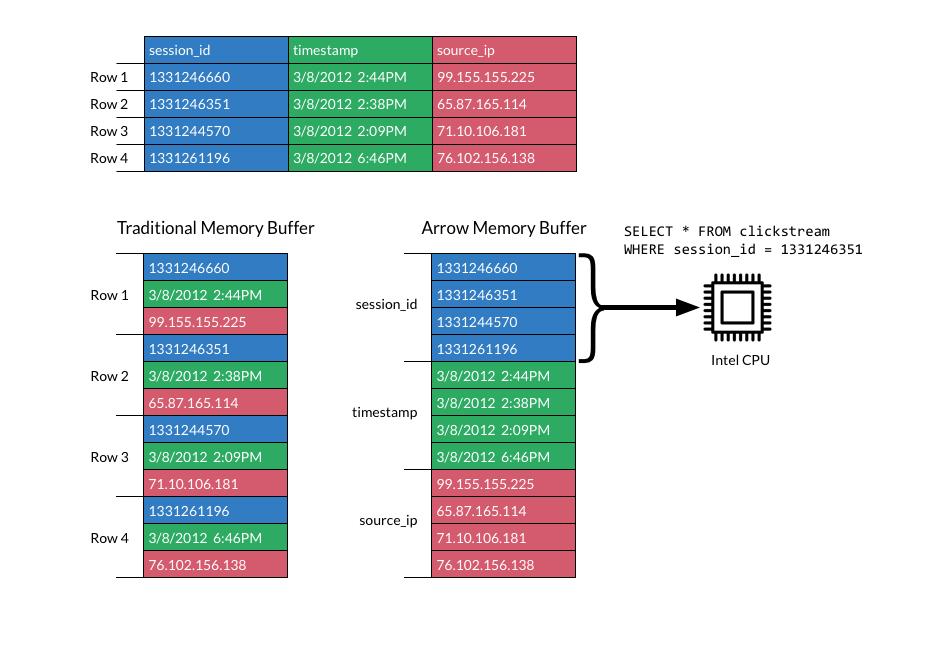
\includegraphics[width=0.95\textwidth]{resources/columnar}
	\end{center}
	\caption{\textbf{Top:} An example table \textbf{Left:} The table in row oriented memory \textbf{Right:} The table in columnar memory}
	\label{fig:row_v_col}
\end{figure}


\section{Columnar Formats}
\label{section:columnar}
Starting around 2011, multiple proposals for a columnar data layour began appearing, resulting in the creation of Apache Parquet and Apache ORC, both disk-based columnar formats.

\section{Apache Arrow}
\label{section:arrow}
"The Apache Arrow project was initiated by the Apache Foundation in 2016.
This framework provides an open and a common standardized format for different programming languages for reading/writing tabular data in-memory.
Through language-specific libraries, multiple languages can share data without any copying or serialization." \autocite{Ahmad2020} (see \ref{fig:arrow_com})
"In the Arrow format, data entries (records) are stored in a table called a RecordBatch.
Each record field is stored in a separate column of the RecordBatch table in a manner that is as contiguous as possible in memory.
This is called an Arrow Array which can store data of different types — i.e., int, float, strings, binary, timestamps and lists, but also nested types (such as lists of lists, etc.).
Arrays may have different types of physical buffers to store data.
This layout provides higher spatial locality when iterating over column contiguous data entries for better CPU cache performance.
SIMD (Single instruction, multiple data) vector operations can also benefit from such a layout as vector elements are already aligned properly in memory." \autocite{Ahmad2020}

- language agnostic in memory format for table like data.
- implementations in many languages exist. %TODO list languages
- record batches (tables) are made up of arrays (columns).
- arrays have:
- data,type
- sequence of buffers (conrtinuous memory region)
- lenght
- null count
- the schema defines fields (columns), each with a name and a datatype
- advantages:
- makes better use of the cache for column based operations
- cite plaintext above
- created in 2016

- more types than javascript -> allows more granular control over memory
- well defined physical layout for each type
- number:
- unsigned integer with fixed width
- signed ""
- decimal(width, scale percision)
- floating point with fixed prercision
- array:
- fixed-size list
- list (32-bit offset), largelist (64bit offset)

\begin{figure}
	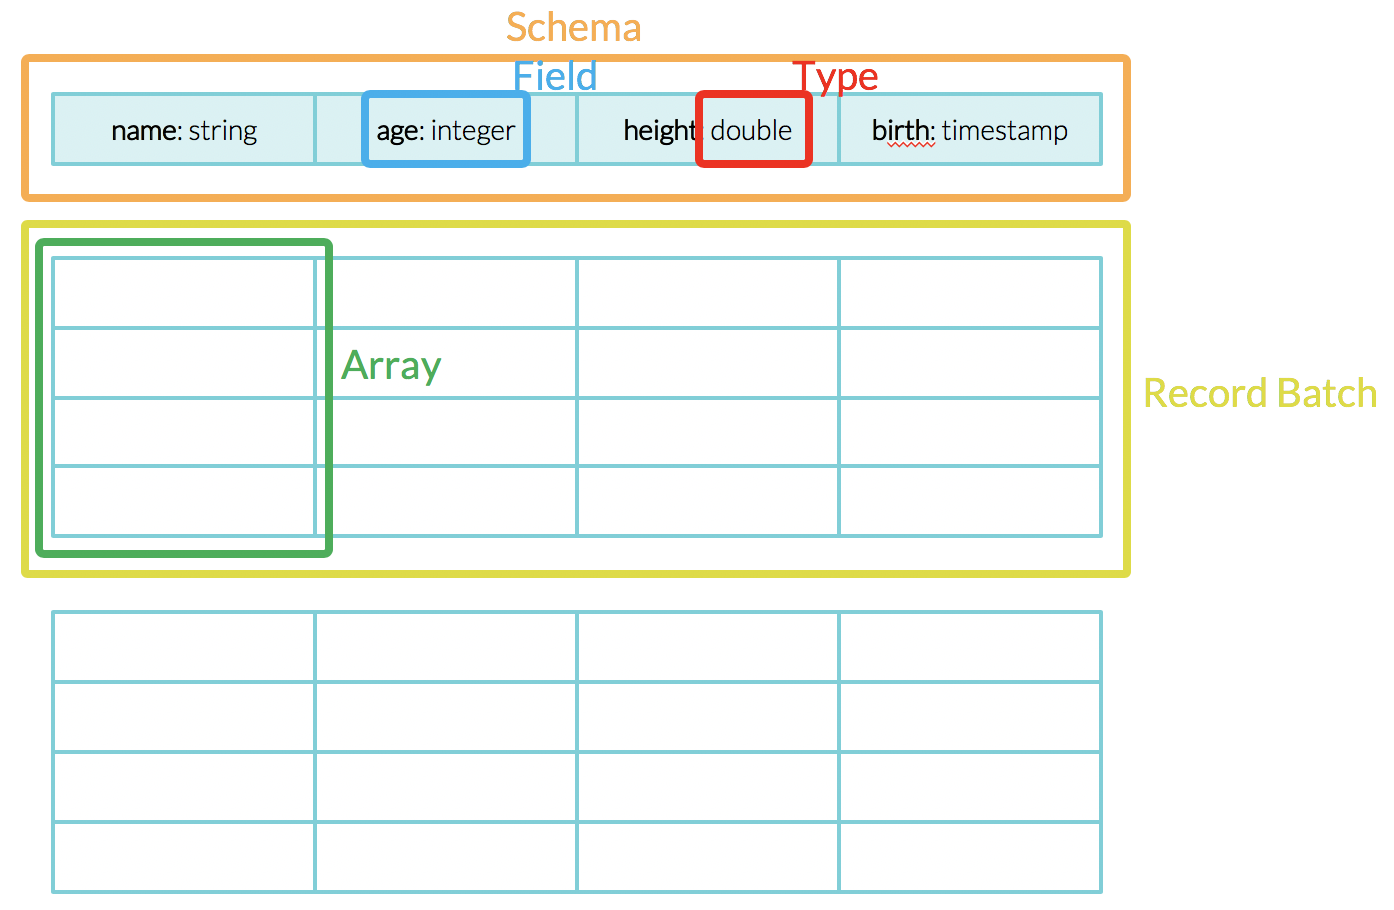
\includegraphics[width=\textwidth]{resources/arrow_tab}
	\caption{Key Concepts of an Arrow Table \autocite{Dremio}}
	\label{fig:arrow_tab}
\end{figure}
\begin{figure}
	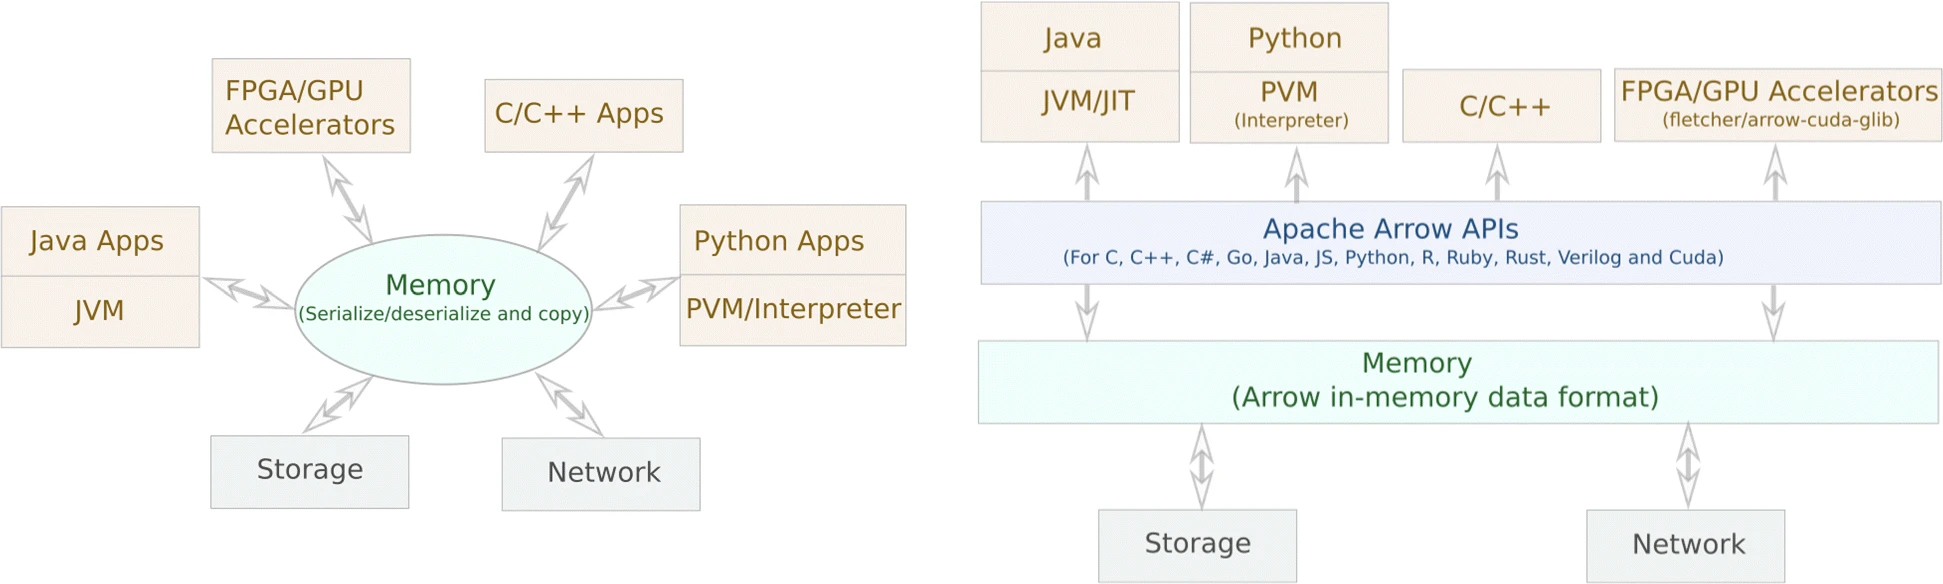
\includegraphics[width=\textwidth]{resources/arrow_interop}
	\caption{Example how Arrow increases interoperability between proceses \autocite{Ahmad2020}}
	\label{fig:arrow_com}
\end{figure}

Apache Arrow has implementations in many languages, including Typescript and Rust \autocite{arrow:status}.
At the time of writing there are 48 projects powered by Apache Arrow \autocite{arrow:projects}.
One of those is Polars.


\section{Napi-rs}
- napi-rs allows us to compile a rust library to a .node file
- nodejs can load and use this .node file
- the types that can be passed to this function is restricted by napi.rs capabilites


\section{Polars}
\label{section:polars}

- implemnents the apache arrow format,
- adds abstractions on top like dataframes
- promises 50x the performance
Polars not only implements the apache arrow format, but adds convenient abstractions like dataframes and series and promises a drastic performance increase.

